\documentclass[oneside, 11pt]{article}

\usepackage[T1]{fontenc}
\usepackage[utf8]{inputenc}
\usepackage[dutch]{babel}

\usepackage{fouriernc}
\usepackage[detect-all, load-configurations=binary,
            separate-uncertainty=true, per-mode=symbol,
            retain-explicit-plus, range-phrase={ tot }]{siunitx}

\usepackage{setspace}
\setstretch{1.2}

\setlength{\parskip}{\smallskipamount}
\setlength{\parindent}{0pt}

\usepackage{geometry}
\geometry{marginparwidth=0.5cm, verbose, a4paper, tmargin=3cm, bmargin=3cm, lmargin=2cm, rmargin=2cm}

\usepackage{float}

\usepackage[fleqn]{amsmath}
\numberwithin{equation}{section}
\numberwithin{figure}{section}

\usepackage{graphicx}
\graphicspath{{Figures/}}
\usepackage{subfig}

\usepackage{tikz}
\usetikzlibrary{plotmarks}

\usepackage{fancyhdr}
\pagestyle{fancy}
\fancyhf{}
\rhead{\thepage}
\renewcommand{\footrulewidth}{0pt}
\renewcommand{\headrulewidth}{0pt}

\usepackage{relsize}
\usepackage{xspace}
\usepackage{url}

\newcommand{\figref}[1]{Figuur~\ref{#1}}

\newcommand{\hisparc}{\textsmaller{HiSPARC}\xspace}
\newcommand{\kascade}{\textsmaller{KASCADE}\xspace}
\newcommand{\sapphire}{\textsmaller{SAPPHiRE}\xspace}
\newcommand{\jsparc}{\textsmaller{jSparc}\xspace}
\newcommand{\hdf}{\textsmaller{HDF5}\xspace}
\newcommand{\aires}{\textsmaller{AIRES}\xspace}
\newcommand{\csv}{\textsmaller{CSV}\xspace}
\newcommand{\python}{\textsmaller{PYTHON}\xspace}
\newcommand{\corsika}{\textsmaller{CORSIKA}\xspace}
\newcommand{\labview}{\textsmaller{LabVIEW}\xspace}
\newcommand{\daq}{\textsmaller{DAQ}\xspace}
\newcommand{\adc}{\textsmaller{ADC}\xspace}
\newcommand{\adcs}{\textsmaller{ADC}s\xspace}
\newcommand{\Adcs}{A\textsmaller{DC}s\xspace}
\newcommand{\hi}{\textsc{h i}\xspace}
\newcommand{\hii}{\textsc{h ii}\xspace}
\newcommand{\mip}{\textsmaller{MIP}\xspace}
\newcommand{\hisparcii}{\textsmaller{HiSPARC II}\xspace}
\newcommand{\hisparciii}{\textsmaller{HiSPARC III}\xspace}
\newcommand{\pmt}{\textsmaller{PMT}\xspace}
\newcommand{\pmts}{\textsmaller{PMT}s\xspace}

\DeclareSIUnit{\electronvolt}{\ensuremath{\mathrm{e\!\!\:V}}}

\DeclareSIUnit{\unitsigma}{\ensuremath{\sigma}}
\DeclareSIUnit{\mip}{\textsmaller{MIP}}
\DeclareSIUnit{\adc}{\textsmaller{ADC}}

\DeclareSIUnit{\gauss}{G}
\DeclareSIUnit{\parsec}{pc}
\DeclareSIUnit{\year}{yr}



\title{Detector plaatsing}
\author{A.P.L.S. de Laat, B. van Eijk} 
\docinstallatie{2}{DP}
\version{1.0}

\begin{document}

\maketitle

\section{Detector plaatsing}

Dit document beschrijft hoe een \hisparc detector op het dak
geïnstalleerd dient te worden.

\textbf{Waarschuwing:} De \hisparc detector met zijn scintillator,
lichtgeleider en \pmt is een fragiel apparaat. Neem daarom de volgende
maatregelen om schade te voorkomen:

\begin{itemize}
    \item Verpak de detector zorgvuldig tijdens transport; de detector
    mag niet kunnen verschuiven in de skibox (voeg extra
    schuimmateriaal toe).
    \item Wanneer de skibox niet horizontaal gehouden kan worden, houd
    de hoge kant van de skibox met de \pmt en kabeldoorvoer, altijd
    boven. Ondersteun de onderkant van de scintillator tegen verschuiven.
    \item Wanneer de detector buiten de skibox verplaatst moet worden,
    zorg er dan voor dat de scintillator en lichtgeleider op voldoende
    plaatsen ondersteund worden om zo breuk in de lijmverbindingen te
    voorkomen.
    \item Voorkom grote schokken aan de \pmt of stoten aan andere
    objecten.
    \item Fixeer de \pmt kabels en connectors met tape (bijv. papieren
    schilderstape) op de licht-geleider zodat geen trekbelasting op de
    draden (en \pmt) kan ontstaan.
\end{itemize}


\section{Aanwijzingen bij de installatie van \hisparc detectoren}

De \hisparc detectoren zijn ondergebracht in skiboxen die bij normaal
gebruik geschikt zijn voor toepassing onder uiteenlopende
weersomstandigheden. De boxen verkrijgen hun stabiliteit door ze via hun
standaard bevestigingspunten (4 beugels) vast te zetten en de deksels op
de juiste wijze te sluiten (scharnieren en 3-punts sluiting) en te
vergrendelen (sleutel + slot). Om er voor te zorgen dat de boxen ook
onder extreme weersomstandigheden (storm) op hun plek blijven, is
gekozen voor een robuuste ‘verankering’. Deze verankering blijft los van
het dak zodat er geen aanpassingen aan het dak zelf noodzakelijk zijn.
Het totale gewicht (en dus de lokale dakbelasting) neemt daardoor wel
toe, maar blijft door een goede gewichtsverdeling beperkt (minder dan
\SI{50}{\kilo\gram\per\square\meter}).

Voordat de skiboxen met hun detectoren definitief geplaatst kunnen
worden moeten diverse elektrische tests uitgevoerd worden en moet de
volledige documentatie voor de opstelling beschikbaar zijn zowel op
papier als op de lokale (school/instituut) website. Dit is de
verantwoordelijkheid van de groep leerlingen die aan de bouw en
plaatsing deelneemt. Met behulp van deze documentatie kunnen de
resultaten van de individuele metingen aan de scintillator,
fotoversterkerbuis en uitleeselektronica gecombineerd worden. Dit is
noodzakelijk om later de signalen van de kosmische straling te kunnen
interpreteren!

Voordat de skiboxen geplaatst worden is het raadzaam om de volgende
punten stap voor stap te controleren:

\begin{itemize}
    \item Iedere detector heeft een sticker met een
    detector-identificatienummer. Dit unieke identificatienummer wordt
    ook in de analyse software gebruikt en wordt aangegeven op de
    statuspagina van de betreffende cluster op de \hisparc website en in
    het logboek van de detector. Dit nummer is ook verbonden met het
    serienummer van de fotoversterker buis.
    \item Om te voorkomen dat tijdens het transport de fotobuis
    beschadigt, wordt de detector zo in de skibox geplaatst dat de
    fotoversterkerbuis zich altijd aan de hogere kant van de skibox
    bevindt (aan dezelfde kant als de kabeldoorvoer).
    \item Voor iedere detector is een volledige elektrische test
    uitgevoerd en gedocumenteerd (kopie rapport bij school in het
    logboek, bij coördinerende instelling en geplaatst op lokale
    webpagina’s).
    \item Iedere detector is gekalibreerd (documentatie: in logboek,
    kopie bij school en bij coördinerende instelling en op
    webpagina’s!).
    \item 1 signaalkabel (coax) en 1 voedingkabel (5-aders) per skibox
    zijn getest en aangelegd (de standaard - maximale - kabellengte is
    \SI{30}{\meter}). De kabels dragen aan beide uiteinden merktekens.
    Let op bij de aanleg: de voedingskabels zijn niet symmetrisch, de
    uiteinden hebben verschillende connectors (male/female)! De fotobuis
    bezit een ‘male’ connector en moet dus verbonden worden met de
    ‘female’ connector van de voedingskabel...
    \item De kabels in de ‘vrije natuur’ (op het dak en langs de gevel)
    zijn bij voorkeur in vast gemonteerde stabiele
    (metalen/kunststoffen) kabelgoten/buizen ondergebracht (de
    voedingsspanning van de fotobuis bedraagt \SI{12}{\volt} met beperkte
    belastbaarheid). Voorkom kortsluiting; bescherm de connectors
    tegen mechanische belasting en inwerking van vocht en voorkom
    scherpe knikken in de kabels!
    \item De \gps antenne is op een stabiele mast of antennevoet in de
    directe nabijheid van het detectiestation geplaatst, zodat de
    antenne ‘vrij zicht’ heeft op een zo groot mogelijk deel van de
    hemel. Bij correcte plaatsing, worden meer dan 5 satellieten
    gelijktijdig waargenomen.
    \item De \gps antenne wordt op een buis/standaard gemonteerd waarbij
    de antenne aan de onderzijde past op een gasfitting van 3⁄4" of
    direct op de bijgeleverde kunststof voet.
    \item De \gps antennekabel is bij voorkeur in een stabiele kabelgoot
    gemonteerd (de \gps kabellengte bedraagt eveneens \SI{30}{\meter};
    deze kabellengte mag zonder speciale maatregelen niet veranderd
    worden!). De kabel heeft aan beide zijden dezelfde connector en mag
    niet los liggen/hangen, vooral niet langs een mast (gebruik
    kabelbinders)!
    \item Er wordt rekening gehouden met speciale
    voorschriften/voorzieningen bij dakbeveiliging tegen blikseminslag.
\end{itemize}


\section{Positie van detectoren en \gps antenne}

Twee verschillende \hisparc detector configuraties worden toegepast; een
twee-skibox opstelling en een vier-skibox opstelling. De opstelling met
twee skiboxen is bij uitstek geschikt wanneer het station gecombineerd
wordt met andere stations in de directe omgeving (cluster centra). Het
totale detectieoppervlak van dit station bedraagt 0.5 + 0.5 = 1.0 m2. Om
de hoekafhankelijkheid van de opstelling te beperken, worden beide
skiboxen parallel geplaatst (de effectieve ‘lengte’ van het station in
twee richtingen is dan \SI{1}{\meter}). De ‘typische’ afstand tussen de
twee skiboxen bedraagt 5 à 6 meter.

De \gps kan tussen de twee skiboxen op de hartlijn van de scintillatoren
geplaatst worden. Meet de Noord-Zuid oriëntatie van deze
hartlijn met een kompas en maak een situatieschets. Een opstelling met 4
detectoren biedt de mogelijkheid om de richting van een lokale
deeltjeslawine te bepalen. Ook hier is gekozen voor een opstelling
waarbij de geometrie geoptimaliseerd is voor symmetrie; drie
detectoren vormen de hoekpunten van een gelijkzijdige driehoek (met
zijden van 10 m). De vierde detector bevindt zich in het zwaartepunt van
deze driehoek. Wanneer in alle vier de detectoren een signaal gemeten
wordt, kunnen in totaal 4 driehoeken onderscheiden worden; triangulatie
- om de richting van de deeltjes te bepalen - kan zo 4 keer uitgevoerd
en op consistentie getest worden...

De \gps kan in het midden op de hartlijn tussen de scintillatoren 3 en 4
geplaatst worden. Wordt van deze positie afgeweken, dan moet een
detailschets gemaakt worden van de positie van de \gps ten opzichte van
de detectoren. Ook hier moet de oriëntatie van de hartlijn tussen 3 en
4 t.o.v. het Noorden met een kompas bepaald worden, De volgorde in de
nummering van de detectoren is eenduidig en mag niet veranderd worden
(Master: scintillator 1 en 2 en Slave: scintillator 3 en 4)!


\section{Installatie van de skiboxen}

Denk aan de voorschriften m.b.t. werken op (platte) daken (o.a. blijf
meer dan 2 meter van de dakrand verwijderd!).

\begin{itemize}
    \item Wees extreem voorzichtig met de detector; de lijmverbindingen
    (scintillator/lichtgeleider, lichtgeleider/fotobuis) zijn fragiel
    en kunnen snel breken waardoor de fotobuis onherstelbaar beschadigd
    kan raken.
    \item Niet boren in de bodem van en/of extra gaten maken in de
    skibox (behalve voor de kabeldoorvoer aan de hoge zijde van de
    skibox). De doorvoer wordt in de box gemonteerd (alleen de moer
    onder in de foto komt aan de buitenkant van de box).
    \item Geen extra gewichten in de skibox plaatsen.
    \item Let op dat bij het transport van de skiboxen deze op de juiste
    wijze (3 punten!) gesloten zijn (en op slot!) terwijl voldoende
    schuimmateriaal is aangebracht om het verschuiven van de
    scintillatieplaat en lichtgeleider te voorkomen (laat de sleutel
    nooit in het slot van de skibox zitten, de sleutel kan eenvoudig
    afbreken!).
    \item Transporteer de detector bij voorkeur horizontaal; bij niet
    horizontale verplaatsing van de detector moet de
    fotobuis zich steeds aan de hoogste zijde bevinden!
    \item Verwijder het schuimmateriaal dat voor transport
    boven de scintillatieplaat en lichtgeleider aan is gebracht pas
    dan wanneer de skibox op zijn definitieve plek geplaatst is.
    \item Meet de precieze afstand tussen de \gps-antenne en de skiboxen
    en maak een positie schets waarbij de Noord-Zuid oriëntatie van de
    skiboxen m.b.v. een kompas bepaald wordt. Neem de schets op in het
    logboek en plaats deze informatie op de lokale webpagina’s.
\end{itemize}


\section{De plaatsing van de skiboxen}

De skiboxen worden gefixeerd via hun standaard bevestigingspunten zodat
de belasting van de bevestigingspunten identiek is aan de belasting op
een autodak. Alleen zo kan veilige montage gegarandeerd worden. Er
worden twee series skiboxen toegepast die qua afmetingen niet
verschillen, maar wel afwijken in de manier waarop de
bevestigingsbeugels in de box gefixeerd worden. Bij de eerste serie -
oudere - skiboxen worden standaard 4 beugels en 4 beugelvergrendelingen
bij iedere skibox geleverd. Voordat de beugels via de onderzijde van de
box in de vergrendeling worden geschoven is het handig om de detector
uit de box te nemen en tijdelijk los op schuimplastic op het dak te
leggen.

De vergrendelingen worden op rails aan de binnenzijde van de skibox zo
ver mogelijk uit elkaar geschoven. De beugels zijn in hoogte
verstelbaar. Op de foto is de ‘vergrendeling’ in ‘ontgrendelde’ toestand
weergegeven, door het centrale deel rechtsom te draaien worden de
beugels vastgeklemd en kan de rode zekering over het uiteinde van het
draaiende deel geschoven worden. Bij de tweede serie – nieuwere –
skiboxen worden standaard 4 beugels, 4 rubberen afdekplaatjes, 4
kunststof afdekplaatjes en 8 moeren geleverd. De beugels worden van
onder in de gaten in de bodem van de skibox geplaatst (kies hiervoor
wederom de gaten die het verste van elkaar verwijderd zijn). Vervolgens
worden aan de binnenzijde van de box de rubberen en kunststof afdekplaat
(in deze volgorde!) over de uiteinden van de beugel geschoven. Tenslotte
worden de moeren op de uiteinden van de beugel gedraaid. De niet
gebruikte gaten in de bodem van de skibox worden met meegeleverde
(zwarte) plastic stickers afgedekt.

Voor de ‘verankering’ van één skibox op het dak zijn de volgende
onderdelen nodig; afwijken van deze methode van plaatsing
wordt ontraden en gebeurt op eigen risico!:

\begin{itemize}
    \item 8 stuks (100 x 15 x 5 cm) of 4 stuks (100 x 30 x 5 cm)
    betonnen opsluitbanden.
    \item 2 kokerprofielen (200 x 5 x 2,5 cm RVS of aluminium) om de
    bevestigingsbeugels te fixeren.
    \item Ongeveer \SI{8}{\meter} RVS-band (‘Bandit’, 3/4 inch breedte)
    met 8 3/4 inch sluitstukken.
\end{itemize}

Afhankelijk van de dakbedekking kunnen rubberen matten of een aantal
rubberen tegels aange- bracht worden waarop de betonnen opsluitbanden
geplaatst kunnen worden. Het RVS band wordt met een spantang om de
kokerbalk en betonnen opsluitbanden gesnoerd. De kokerbalken drukken de
twee beugels tegen de opsluitbanden. De beugels steken door de bodem van
de skibox. De vergrendelingen/moeren op de beugels aan de binnenzijde
van de skibox zorgen ervoor dat de skibox op de kokerbalk gefixeerd
wordt. Het sluitstuk van de band is eveneens van RVS (linksonder) en
heeft vertandingen en sluitnokken (rechtsboven) waarmee de band
gefixeerd wordt. De nokken worden met een hamer om de band ‘gebogen’. De
spantang heeft een ingebouwde schaar waarmee de band op lengte kan
worden geknipt. Per skibox worden zo 8 spanbanden aangebracht.

Leg, als alle banden gemonteerd zijn, de detector weer in de skibox. Let
op dat de kabelgoten zo dicht mogelijk bij de skibox eindigen en dat de
kabels langer zijn dan strikt noodzakelijk om de connectors van de
fotobuizen te bereiken. Deze extra kabellengte wordt los in de skibox
(rond de scintillatorplaat) ondergebracht zodat een
eenvoudige ‘trekontlasting’ van de kabel aan de fotobuis ontstaat. De
kabels worden bij de kabeldoorvoer in de skibox voorzien van twee extra
kabelbinders (die niet afgeknipt worden!). Zo wordt een extra
trekontlasting verkregen. Iedere detectieopstelling bezit twee sets
sleutels. Een set wordt beheerd door de school (blauw label); de
reservesleutels worden beheerd door de clustercoördinator (rood label).

Tenslotte, het is uiterst belangrijk dat het deksel van de skibox op de
juiste wijze - d.w.z. het deksel sluit aan alle randen terwijl de
sleutel zonder veel kracht uit te oefenen omgedraaid kan worden -
gesloten wordt! Uiteraard moet er geen schuim bovenop de
scintillator en de lichtgeleider in de skibox achterblijven...

DISCLAIMER: de hier beschreven plaatsingsmethode is ontwikkeld op basis
van de gegevens verstrekt door de fabrikant van de skiboxen en is
geverifieerd door constructeurs. De methode heeft zich in de praktijk
bewezen. Op enigerlei wijze afwijken van deze methode geschiedt
uitdrukkelijk op eigen verantwoordelijkheid en wordt ten sterkste
ontraden!

\begin{figure}
    \centering
    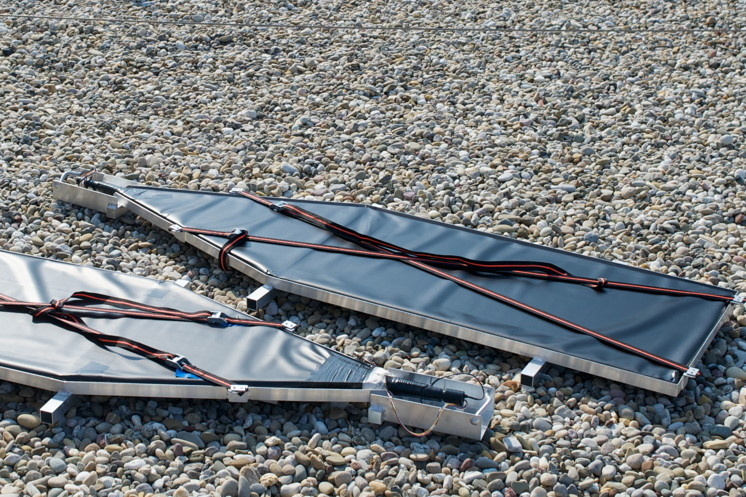
\includegraphics[width=0.47\linewidth]{frames}
    \label{fig:frames}
    \caption{Detectoren in metalen frames voor vervoer.}
\end{figure}

\begin{figure}
    \centering
    \subfloat[]{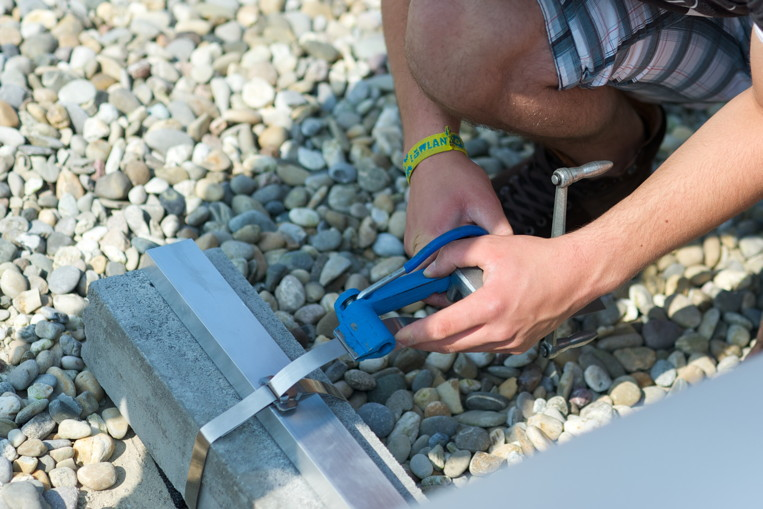
\includegraphics[width=0.47\linewidth]{spanband_spannen}
                \label{fig:spanband_spannen}}
    \subfloat[]{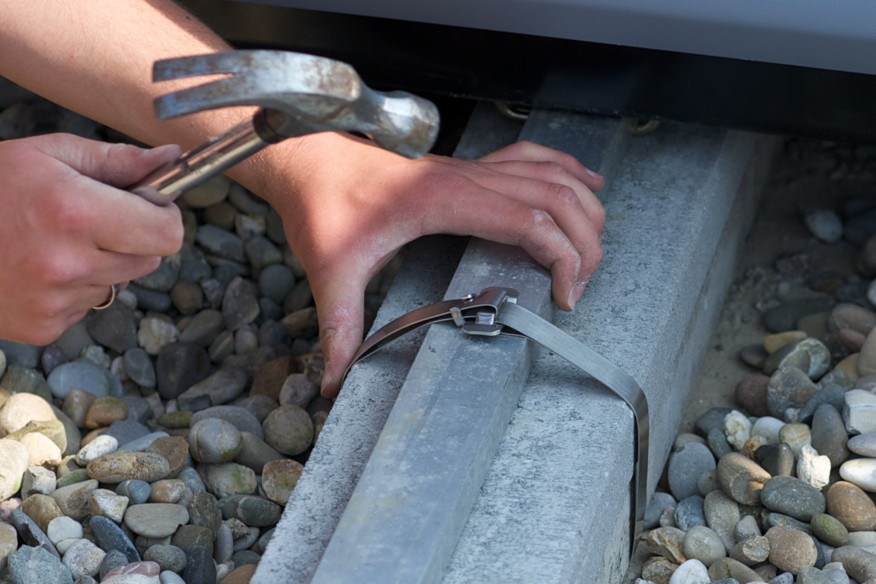
\includegraphics[width=0.47\linewidth]{spanband_verankeren}
                \label{fig:spanband_verankeren}}
    \caption{Spannen van de spanbanden. Verankeren van de spanband}
\end{figure}

\begin{figure}
    \centering
    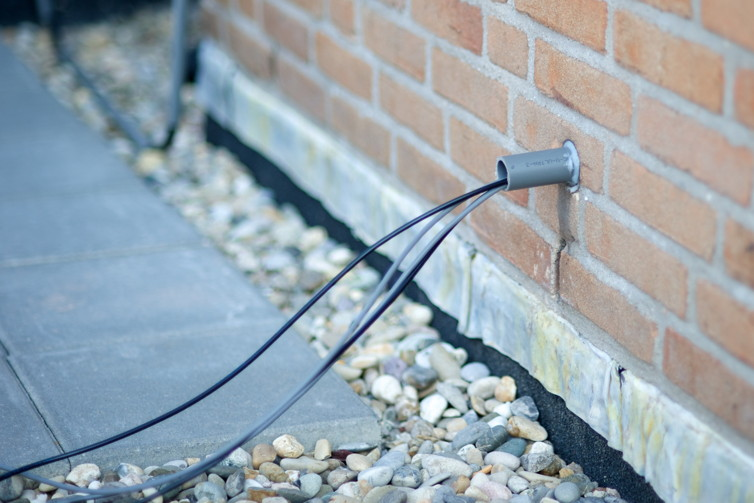
\includegraphics[width=0.47\linewidth]{kabel_doorvoer}
    \label{fig:kabel_doorvoer}
    \caption{Doorvoer in de muur voor de kabels.}
\end{figure}

\begin{figure}
    \centering
    \subfloat[]{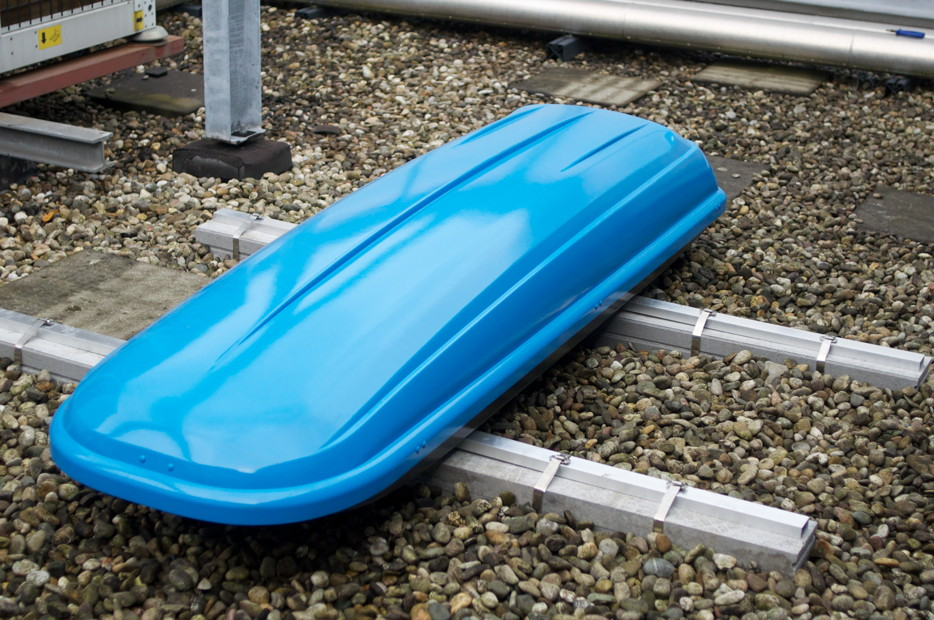
\includegraphics[width=0.47\linewidth]{klaar_skibox}
                \label{fig:klaar_skibox}}
    \subfloat[]{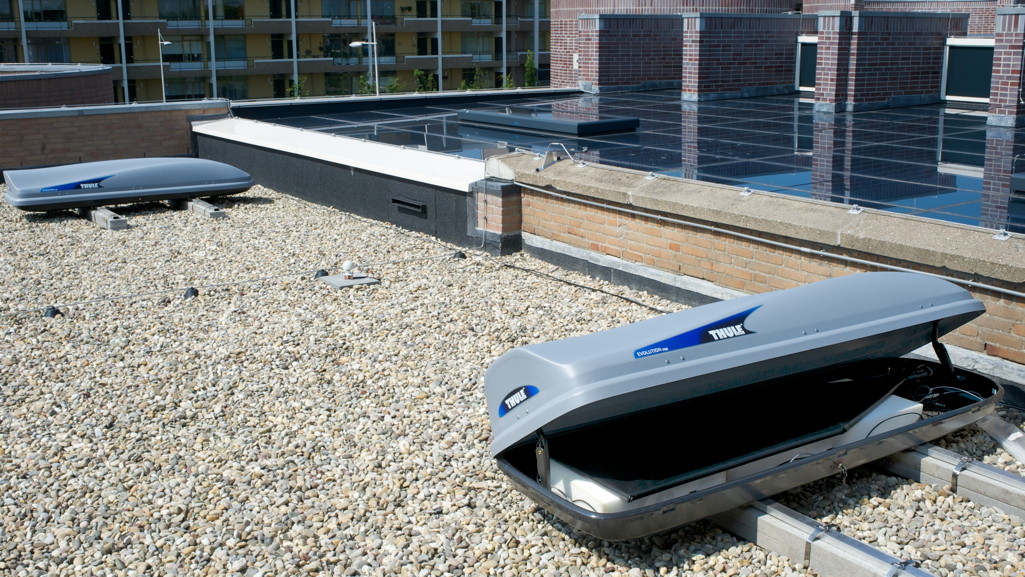
\includegraphics[width=0.47\linewidth]{klaar_station}
                \label{fig:klaar_station}}
    \caption{Geïnstaleerde detector stations.}
\end{figure}

\begin{figure}
    \centering
    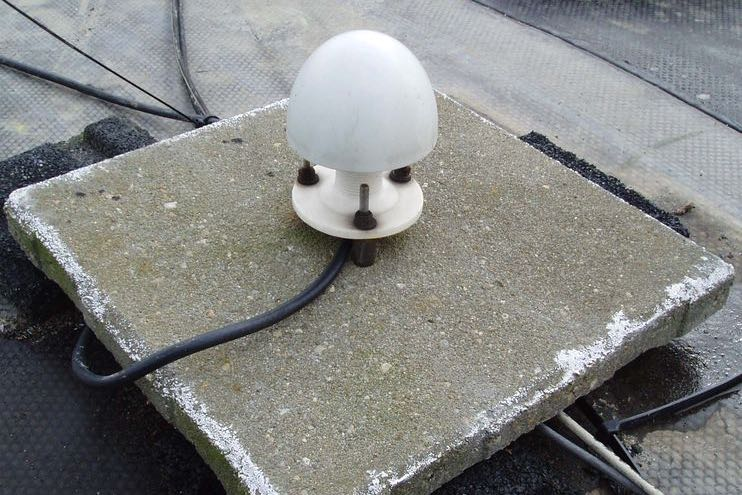
\includegraphics[width=0.47\linewidth]{gps_stoeptegel}
    \label{fig:gps_stoeptegel}
    \caption{\gps bevestigd op voet.}
\end{figure}

%\begin{thebibliography}{9}
%\end{thebibliography}

\end{document}
